\chapter{Endocrinología y homeostasis}\label{ch:b3:endocrinology}

En el verano de 1921, dos hombres jóvenes en un laboratorio caluroso de
Toronto ligaron los conductos pancreáticos de unos perros, esperaron a
que el tejido digestivo se marchitara, molieron lo que quedaba e
inyectaron el extracto en un perro al que habían vuelto diabético
retirándole el páncreas. Su azúcar en sangre bajó. En enero, un
muchacho de catorce años que se moría de diabetes en el Hospital
General de Toronto recibía el extracto, y en pocas semanas comía,
caminaba y ganaba peso; vivió trece años más. La sustancia, la
\omterm{def:b3:endocrinology:glucose}{insulina}, es un péptido de cincuenta y un aminoácidos que segrega el
uno por ciento del páncreas hacia la sangre, donde, a una
concentración de unos cientos de picomolar, dice a todas las células
musculares y adiposas del cuerpo qué hacer con el azúcar de la última
comida. Este capítulo trata de tales mensajeros: qué son, cómo una
célula que jamás ha conocido la glándula sabe qué significa el mensaje,
cómo se gobiernan las propias glándulas en una jerarquía de bucles de
retroalimentación, y cómo el conjunto mantiene la glucosa, la sal, el
calcio y la temperatura de la sangre dentro de un pequeño porcentaje
durante toda una vida ---y qué ocurre, en la clínica, cuando falla uno
de los bucles.

\section{Las hormonas y sus receptores}

\begin{definition}[Hormona]\label{def:b3:endocrinology:hormone}
\index{hormona}\index{glándula endocrina}\index{paracrino}\index{hormona esteroidea}\index{hormona peptídica}\index{receptor nuclear}
Una \emph{hormona} es una sustancia que una célula libera a la sangre y
que actúa sobre células lejanas que llevan su receptor; una señal
\emph{paracrina} actúa sobre las vecinas, una \emph{autocrina} sobre la
propia célula que la fabricó, y una neurohormona la libera una neurona
a la sangre. A las \emph{glándulas endocrinas} clásicas ---hipófisis,
tiroides, paratiroides, suprarrenales, islotes pancreáticos, gónadas---
se han sumado el corazón (péptido natriurético), el riñón
(eritropoyetina), la grasa (leptina), el intestino (una docena de
péptidos) y el hueso. Químicamente hay hormonas de tres clases, y la
química fija el mecanismo. Las \emph{hormonas peptídicas y proteicas}
(\omterm{def:b3:endocrinology:glucose}{insulina}, hormona del crecimiento, las hormonas hipofisarias) se
fabrican en los ribosomas, se almacenan en gránulos, se liberan por
exocitosis, viajan libres por el plasma, no pueden cruzar membranas y
actúan sobre receptores de la superficie celular ---acoplados a
proteínas G o ligados a cinasas--- a través de segundos mensajeros, en
segundos o minutos; sus semividas son de minutos. Los \emph{esteroides}
(cortisol, \omterm{def:b3:renal-osmoregulation:controls}{aldosterona}, estrógenos, testosterona y el secosteroide
\omterm{def:b3:endocrinology:calcium}{vitamina D}) se fabrican a partir del colesterol según hace falta, no se
almacenan, viajan unidos a proteínas transportadoras, cruzan membranas
y se unen a \emph{receptores nucleares} que son ellos mismos factores
de transcripción: sus efectos tardan horas y duran días. Las
\emph{aminas} quedan a caballo entre ambas: la adrenalina actúa en la
superficie en un segundo; las \omterm{prop:b3:endocrinology:thyroid}{hormonas tiroideas}, aun siendo derivados
de aminoácidos, actúan sobre receptores nucleares como los esteroides.
Una hormona no significa nada por sí misma: la misma adrenalina dilata
un vaso y contrae otro porque sus músculos lisos llevan subtipos
distintos de receptor, y el mismo cortisol eleva la glucosa sanguínea
en el hígado y suprime un \omterm{def:b3:adaptive-immunity:lymphocytes}{linfocito} porque la \omterm{def:b3:chromatin-epigenetics:nucleosome}{cromatina} de las dos
células ofrece a su receptor genes distintos.
\end{definition}

\begin{omfigure}
\begin{tikzpicture}[every node/.style={font=\scriptsize}, >=stealth]
  % peptide pathway
  \draw[thick, omDef, fill=omDef!10] (0,0) rectangle (5.2,3.4);
  \node[above] at (2.6,3.4) {hormona peptídica o amina --- receptor de superficie};
  \draw[thick, omDef] (0,2.6) -- (5.2,2.6); \node[left, font=\tiny] at (5.2,2.75) {membrana};
  \node[circle, fill=omThm!60, inner sep=2pt, label={[font=\tiny]right:hormona}] (h1) at (1.4,3.1) {};
  \draw[thick, omDef!80!black, fill=omDef!40] (1.1,2.3) rectangle (1.7,2.9); \node[below, font=\tiny] at (1.4,2.3) {receptor};
  \draw[->, thick] (2.0,2.1) -- (3.0,2.1) node[right, align=left, font=\tiny] {proteína G o\\actividad cinasa};
  \draw[->, thick] (2.6,1.75) -- (2.6,1.25) node[below, align=center, font=\tiny] {AMPc, Ca$^{2+}$, IP$_3$ o\\cascada de fosforilación};
  \draw[->, thick] (2.6,0.55) -- (2.6,0.25) node[below=-2pt, font=\tiny] {enzimas conmutadas: de segundos a minutos};
  % steroid pathway
  \draw[thick, omProp, fill=omProp!10] (6.4,0) rectangle (11.6,3.4);
  \node[above] at (9.0,3.4) {hormona esteroidea o tiroidea --- receptor nuclear};
  \draw[thick, omProp] (6.4,2.6) -- (11.6,2.6);
  \node[circle, fill=omMeth!70, inner sep=2pt, label={[font=\tiny]right:hormona sobre su transportador}] (h2) at (7.6,3.1) {};
  \draw[->, thick] (7.6,2.95) -- (7.6,2.2) node[below, font=\tiny] {difunde a través};
  \draw[->, thick] (7.9,1.85) -- (9.0,1.5); \draw[thick, omProp!80!black, fill=omProp!35] (8.8,1.0) rectangle (9.6,1.7); \node[right, align=left, font=\tiny] at (9.65,1.35) {complejo hormona--receptor,\\un factor de\\transcripción};
  \draw[thick, omProp] (7.0,0.2) rectangle (11.0,0.8); \node[font=\tiny] at (9.0,0.5) {núcleo: genes encendidos o apagados --- de horas a días};
  \draw[->, thick] (9.2,1.0) -- (9.2,0.82);
\end{tikzpicture}

{\small Dos maneras de oír una \omterm{def:b3:endocrinology:hormone}{hormona}. Las \omterm{def:b3:endocrinology:hormone}{hormonas} hidrosolubles se
detienen en la superficie y actúan mediante segundos mensajeros, deprisa
y por poco tiempo; las liposolubles entran, se unen a un receptor que es
un factor de transcripción y cambian lo que la célula fabrica, despacio
y por mucho tiempo.}
\end{omfigure}

\begin{proposition}[Dosis y respuesta]\label{prop:b3:endocrinology:dose}
\index{curva dosis--respuesta}\index{receptores de reserva}\index{regulación a la baja}
Una célula con $R$ receptores de constante de disociación $K_{d}$ en
una concentración hormonal $H$ tiene ocupados $R\,H/(K_{d} + H)$ de
ellos, y la respuesta suele crecer con la ocupación a lo largo de una
sigmoide en un eje logarítmico de dosis, semimáxima en una
$\text{EC}_{50}$ que a menudo queda muy por debajo de $K_{d}$: una
ocupación de un pequeño porcentaje da una respuesta completa, porque la
señal se amplifica aguas abajo (un receptor activa muchas proteínas G,
una cinasa fosforila muchos sustratos), y el excedente de
\emph{\omterm{prop:b3:endocrinology:dose}{receptores de reserva}} desplaza la curva a la izquierda y vuelve
sensible a la célula a dosis bajas. La célula ajusta su propia
sensibilidad: una exposición prolongada a una \omterm{def:b3:endocrinology:hormone}{hormona} retira sus
receptores de la superficie (\emph{\omterm{prop:b3:endocrinology:dose}{regulación a la baja}}), que es el
mecanismo por el cual una \omterm{def:b3:endocrinology:glucose}{insulina} persistentemente alta embota el
efecto de la propia \omterm{def:b3:endocrinology:glucose}{insulina}; la privación los aumenta. Las \omterm{def:b3:endocrinology:hormone}{hormonas}
circulan de $10^{-12}$ a $10^{-9}$ molar ---de mil a un millón de veces
por debajo de la mayoría de los metabolitos---, y por eso los
receptores han de unirlas con afinidad nanomolar, y por eso medirlas
exigió un método nuevo.
\end{proposition}
\begin{proof}
La ocupación es la isoterma de acción de masas de un único sitio de
unión. Si la respuesta se satura cuando hay ocupados $n \ll R$
receptores, entonces es semimáxima cuando $R H/(K_{d} + H) = n/2$, es
decir, $H = K_{d}\,
(n/2)/(R - n/2) \approx K_{d}\, n/(2R) \ll K_{d}$: la EC$_{50}$ cae en
proporción al exceso de receptores. Perder receptores la eleva, que es
el efecto de la \omterm{prop:b3:endocrinology:dose}{regulación a la baja} sobre la curva.
\end{proof}

\begin{method}[Radioinmunoanálisis]\label{met:b3:endocrinology:ria}
\index{radioinmunoanálisis}\index{inmunoanálisis}
Para medir una \omterm{def:b3:endocrinology:hormone}{hormona} a concentración picomolar (Yalow y Berson,
1959): (1) prodúzcase un \omterm{def:b3:adaptive-immunity:antibody}{anticuerpo} contra ella; (2) mézclese una
cantidad pequeña y fija de \omterm{def:b3:adaptive-immunity:antibody}{anticuerpo} con una cantidad fija de \omterm{def:b3:endocrinology:hormone}{hormona}
marcada radiactivamente, y añádase la muestra; (3) la \omterm{def:b3:endocrinology:hormone}{hormona} sin
marcar de la muestra compite con la marcada por los sitios del
\omterm{def:b3:adaptive-immunity:antibody}{anticuerpo}, de modo que cuanta más \omterm{def:b3:endocrinology:hormone}{hormona} contiene la muestra, menos
marca queda unida; (4) sepárese la marca unida de la libre y cuéntese;
(5) léase la concentración de la muestra en una curva patrón hecha con
cantidades conocidas. Sus descendientes sustituyen el isótopo por una
enzima o un fluoróforo y emplean dos \omterm{def:b3:adaptive-immunity:antibody}{anticuerpos} (un ``sándwich'') para
ganar especificidad; miden todas las \omterm{def:b3:endocrinology:hormone}{hormonas} de este capítulo a partir
de una gota de sangre, e hicieron de la endocrinología una ciencia
cuantitativa.
\end{method}

\section{La jerarquía: hipotálamo e hipófisis}

\begin{definition}[Los ejes]\label{def:b3:endocrinology:axes}
\index{hipotálamo}\index{hipófisis}\index{sistema porta}\index{hormona liberadora}\index{hormona trópica}\index{retroalimentación negativa}
El \emph{hipotálamo}, unos pocos gramos de encéfalo situados encima de
la hipófisis, convierte la información neural ---el estrés, el frío, la
duración del día, la \omterm{def:b3:renal-osmoregulation:problem}{osmolaridad} y la glucosa de la sangre--- en
órdenes hormonales. Sus células neurosecretoras liberan \emph{\omterm{def:b3:endocrinology:hormone}{hormonas}
liberadoras} (péptidos: CRH, TRH, GnRH, GHRH, y el inhibidor
somatostatina; dopamina para la prolactina) a un \emph{sistema porta}
privado de vasos que las lleva, sin diluir, un centímetro más abajo
hasta la \emph{adenohipófisis}, cuyas células responden con
\emph{\omterm{def:b3:endocrinology:hormone}{hormonas} trópicas}: ACTH a la corteza suprarrenal, TSH a la
tiroides, LH y FSH a las gónadas, \omterm{def:b3:endocrinology:hormone}{hormona} del crecimiento al hígado y
a los tejidos, prolactina a la mama. Las \omterm{def:b3:endocrinology:hormone}{hormonas} de las glándulas
diana ---cortisol, tiroxina, esteroides sexuales--- retroalimentan
tanto a la hipófisis como al hipotálamo para apagar sus propias
órdenes: \emph{retroalimentación negativa}, en tres pisos. La
\emph{neurohipófisis} no es una glándula, sino los terminales axónicos
de neuronas hipotalámicas, que liberan vasopresina y oxitocina
directamente a la sangre. Cada eje tiene su propia dinámica: el eje
tiroideo es lento y estable, y mantiene un \omterm{thm:b3:endocrinology:loop}{punto de consigna} durante
años; el eje suprarrenal es pulsátil y circadiano, con el cortisol en
su máximo antes del amanecer y segregado en ráfagas horarias; el eje
gonadal de una mujer recorre un ciclo mensual sobre una
retroalimentación positiva de la que los demás carecen.
\end{definition}

\begin{omfigure}
\begin{tikzpicture}[every node/.style={font=\scriptsize}, >=stealth]
  \node[draw, thick, rounded corners, fill=omDef!20, align=center, minimum width=3.2cm] (hyp) at (0,3.4) {hipotálamo\\CRH, TRH, GnRH, GHRH};
  \node[draw, thick, rounded corners, fill=omDef!20, align=center, minimum width=3.2cm] (pit) at (0,1.7) {adenohipófisis\\ACTH, TSH, LH/FSH, GH};
  \node[draw, thick, rounded corners, fill=omProp!25, align=center, minimum width=3.2cm] (gl) at (0,0) {glándula diana\\cortisol, T$_4$, esteroides sexuales};
  \node[draw, thick, rounded corners, fill=omMeth!25, align=center, minimum width=3.2cm] (tis) at (0,-1.7) {tejidos: efectos};
  \draw[->, very thick] (hyp) -- (pit) node[midway, right, font=\tiny] {vasos porta};
  \draw[->, very thick] (pit) -- (gl) node[midway, right, font=\tiny] {sangre};
  \draw[->, very thick] (gl) -- (tis);
  \draw[-|, thick, omThm] (gl.west) -- ++(-0.9,0) |- (pit.west) node[pos=0.25, left, font=\tiny, omThm, align=right] {bucle\\corto};
  \draw[-|, thick, omThm] (gl.west) ++(-0.9,0) -- ++(-0.7,0) |- (hyp.west) node[pos=0.25, left, font=\tiny, omThm, align=right] {bucle\\largo};
  \node[left, align=right, font=\tiny] at (-2.0,4.4) {entradas: estrés, frío,\\luz, metabolitos};
  \draw[->, thick] (-1.9,4.3) -- (hyp.north west);
  % right: the thyroid example with numbers
  \node[right, align=left] at (3.4,3.4) {eje tiroideo: TRH $\to$ TSH $\to$ T$_4$, T$_3$;\\semivida de T$_4$, 7 días, consigna mantenida años;\\el log de TSH baja linealmente al subir la T$_4$ libre};
  \node[right, align=left] at (3.4,1.7) {eje suprarrenal: CRH $\to$ ACTH $\to$ cortisol;\\pulsos cada 1--2 h, máximo antes de despertar;\\el estrés se impone a la retroalimentación};
  \node[right, align=left] at (3.4,0) {eje gonadal: pulsos de GnRH $\to$ LH, FSH $\to$\\estradiol, progesterona, testosterona;\\un pico de retroalimentación positiva al mes};
  \node[right, align=left] at (3.4,-1.7) {eje del crecimiento: GHRH, somatostatina $\to$ GH $\to$\\IGF-1 del hígado; pulsos por la noche};
\end{tikzpicture}

{\small Los ejes de tres pisos. Las \omterm{def:b3:endocrinology:axes}{hormonas liberadoras} alcanzan la
\omterm{def:b3:endocrinology:axes}{hipófisis} por los vasos porta; la \omterm{def:b3:endocrinology:axes}{hipófisis} manda sobre una glándula; la
\omterm{def:b3:endocrinology:hormone}{hormona} de la glándula apaga los dos pisos de arriba. Cada eje tiene su
propio ritmo y sus propios fallos.}
\end{omfigure}

\begin{proof}[Evidencia]
Berthold (1849) castró gallos, que perdieron la cresta, el canto y la
combatividad; reimplantar un testículo en cualquier punto del abdomen,
sin sus nervios, se los devolvió ---el órgano actuaba por la sangre.
Harris (en los años cincuenta) cortó los vasos porta entre el
\omterm{def:b3:endocrinology:axes}{hipotálamo} y la \omterm{def:b3:endocrinology:axes}{hipófisis} en ratas: la \omterm{def:b3:endocrinology:axes}{hipófisis}, con su riego
restablecido desde otra parte, dejó de responder al estrés y los
ovarios dejaron de ciclar; trasplantar una \omterm{def:b3:endocrinology:axes}{hipófisis} bajo el riñón la
dejaba inerte, pero bajo el \omterm{def:b3:endocrinology:axes}{hipotálamo}, donde los vasos porta volvían a
crecer hacia ella, funcionaba ---el encéfalo gobierna la glándula
mediante factores transportados por la sangre, y Guillemin y Schally
aislaron después el primero de ellos, la TRH, a partir de millones de
\omterm{def:b3:endocrinology:axes}{hipotálamos} de oveja y de cerdo (1969): tres aminoácidos.
\end{proof}

\begin{proposition}[La retroalimentación y la tiroides log-lineal]\label{prop:b3:endocrinology:thyroid}
\index{hormona tiroidea}\index{TSH}\index{hipotiroidismo}\index{hipertiroidismo}\index{bocio}
La tiroides capta yoduro y fabrica tiroxina, T$_{4}$ (cuatro yodos),
que los tejidos convierten en la T$_{3}$ activa; ambas elevan el ritmo
metabólico de casi toda célula, fijan la frecuencia cardíaca y hacen
falta para el desarrollo del encéfalo antes y después del nacimiento.
La TSH de la \omterm{def:b3:endocrinology:axes}{hipófisis} impulsa tanto la síntesis como el crecimiento de
la glándula; la T$_{4}$ suprime la TSH. La relación en estado
estacionario es \emph{log-lineal}: el logaritmo de la TSH baja en
proporción a la T$_{4}$ libre,
\[
\text{TSH} = \text{TSH}_{0}\,\mathrm{e}^{-\kappa\,(T_{4} - T_{4,0})},
\]
de modo que una caída de un tercio de la T$_{4}$ libre eleva la TSH
unas diez veces ---por eso la TSH, y no la T$_{4}$, es la prueba
sensible: una glándula que empieza a fallar muestra una T$_{4}$ normal
sostenida por una TSH ya varias veces normal. El fallo de la glándula
(destrucción autoinmunitaria, carencia de yodo) da \emph{hipotiroidismo}
---frío, lento, cansado, con una TSH alta y, en la carencia de yodo,
una glándula agrandada hasta el \emph{bocio} por la TSH que no logra
hacerla producir; un \omterm{def:b3:adaptive-immunity:antibody}{anticuerpo} que imita a la TSH da
\emph{hipertiroidismo} (enfermedad de Graves), con un paciente
acalorado, acelerado y delgado y una TSH suprimida hasta nada, ya que
la estimulación escapa a la retroalimentación. Un recién nacido sin
\omterm{prop:b3:endocrinology:thyroid}{hormona tiroidea} desarrolla una discapacidad intelectual irreversible
en pocos meses, y por eso se mide la TSH de todo recién nacido en una
gota de sangre.
\end{proposition}
\begin{proof}
La producción de TSH de la célula hipofisaria responde a la ocupación
del receptor por la T$_{3}$, proporcional ella misma a la T$_{4}$, y la
respuesta de una represión transcripcional a un cambio de ocupación es
multiplicativa ---cada incremento de \omterm{def:b3:endocrinology:hormone}{hormona} reprime la misma fracción
de lo que queda---, de modo que
$\mathrm{d}\ln\text{TSH}/\mathrm{d}T_{4} = -\kappa$, de donde sale la
exponencial. Con $\kappa$ ajustada para que una $T_{4}$ que cae de
$15$ a \qty{10}{pmol/L} eleve la TSH de $1.5$ a \qty{15}{mU/L},
$\kappa = \ln 10/5 = \qty{0.46}{L/pmol}$: la TSH se duplica por cada
\qty{1.5}{pmol/L} de T$_{4}$ perdida, que es la amplificación que la
convierte en la prueba sensible.
\end{proof}

\begin{omfigure}
\begin{tikzpicture}
\begin{semilogyaxis}[
  width=0.6\linewidth, height=5.6cm,
  axis x line=bottom, axis y line=left,
  xmin=4, xmax=30, ymin=0.02, ymax=200,
  xlabel={T$_4$ libre (pmol/L)}, ylabel={TSH (mU/L)},
  xlabel style={font=\small, at={(axis description cs:0.5,-0.12)}, anchor=north}, ylabel style={font=\small},
  tick label style={font=\small}, xtick={5,10,15,20,25,30}, ytick={0.1,1,10,100},
  yticklabels={0.1,1,10,100},
  clip=false,
]
\addplot[very thick, omDef, domain=4.5:24.4, samples=60] {1.5*exp(-0.46*(x-15))};
\fill[omProp, opacity=0.15] (axis cs:10,0.4) rectangle (axis cs:20,4);
\node[font=\scriptsize, omProp!80!black, anchor=south] at (axis cs:15,4.2) {intervalo de referencia};
\node[font=\scriptsize, omThm, anchor=north west, align=left] at (axis cs:12,150) {glándula que falla:\\TSH alta, T$_4$ aún normal};
\node[font=\scriptsize, omMeth!70!black, anchor=south west, align=left] at (axis cs:22,0.5) {enfermedad de Graves:\\T$_4$ alta, TSH suprimida};
\end{semilogyaxis}
\end{tikzpicture}

{\small El \omterm{thm:b3:endocrinology:loop}{punto de consigna} de la tiroides visto desde fuera. Como el
logaritmo de la TSH baja linealmente con la T$_4$, una pequeña caída de
la \omterm{def:b3:endocrinology:hormone}{hormona} produce una gran subida de la orden ---la \omterm{def:b3:endocrinology:axes}{hipófisis} es un
amplificador logarítmico del fallo de la glándula.}
\end{omfigure}

\begin{example}[El cortisol: el eje del estrés]\label{ex:b3:endocrinology:cortisol}
El cortisol, procedente de la corteza suprarrenal bajo la ACTH,
moviliza combustible (glucosa del hígado, aminoácidos del músculo,
ácidos grasos de la grasa), sensibiliza los vasos a la adrenalina y
suprime la \omterm{def:b3:innate-immunity:inflammation}{inflamación} y la respuesta inmunitaria ---la razón de que
sus parientes sintéticos sean los antiinflamatorios más comunes. Su
ritmo lo fija el reloj: \qty{500}{nmol/L} a las ocho de la mañana, la
quinta parte de eso a medianoche, y pulsos cada una o dos horas a lo
largo de todo el día, ya que las neuronas hipotalámicas de CRH
descargan en ráfagas. El estrés ---hemorragia, infección, cirugía,
miedo--- lo eleva diez veces en minutos, imponiéndose a la
retroalimentación. Demasiado poco (enfermedad de Addison, destrucción
de la corteza suprarrenal) da debilidad, presión arterial baja, glucosa
baja y, bajo estrés, colapso y muerte si no se repone; demasiado
(síndrome de Cushing: un \omterm{def:b3:cancer-biology:hallmarks}{tumor} hipofisario que fabrica ACTH, un \omterm{def:b3:cancer-biology:hallmarks}{tumor}
suprarrenal o, más a menudo, esteroides recetados) da la cara redonda,
la piel fina, el músculo consumido, la glucosa alta, la presión alta y
los huesos frágiles de la exposición prolongada. Interrumpir de golpe
un tratamiento largo con esteroides es peligroso por la razón que el
eje predice: el \omterm{def:b3:endocrinology:axes}{hipotálamo} y la \omterm{def:b3:endocrinology:axes}{hipófisis} suprimidos tardan semanas en
recuperarse, y la suprarrenal, sin estímulo, se ha encogido.
\end{example}

\begin{omfigure}
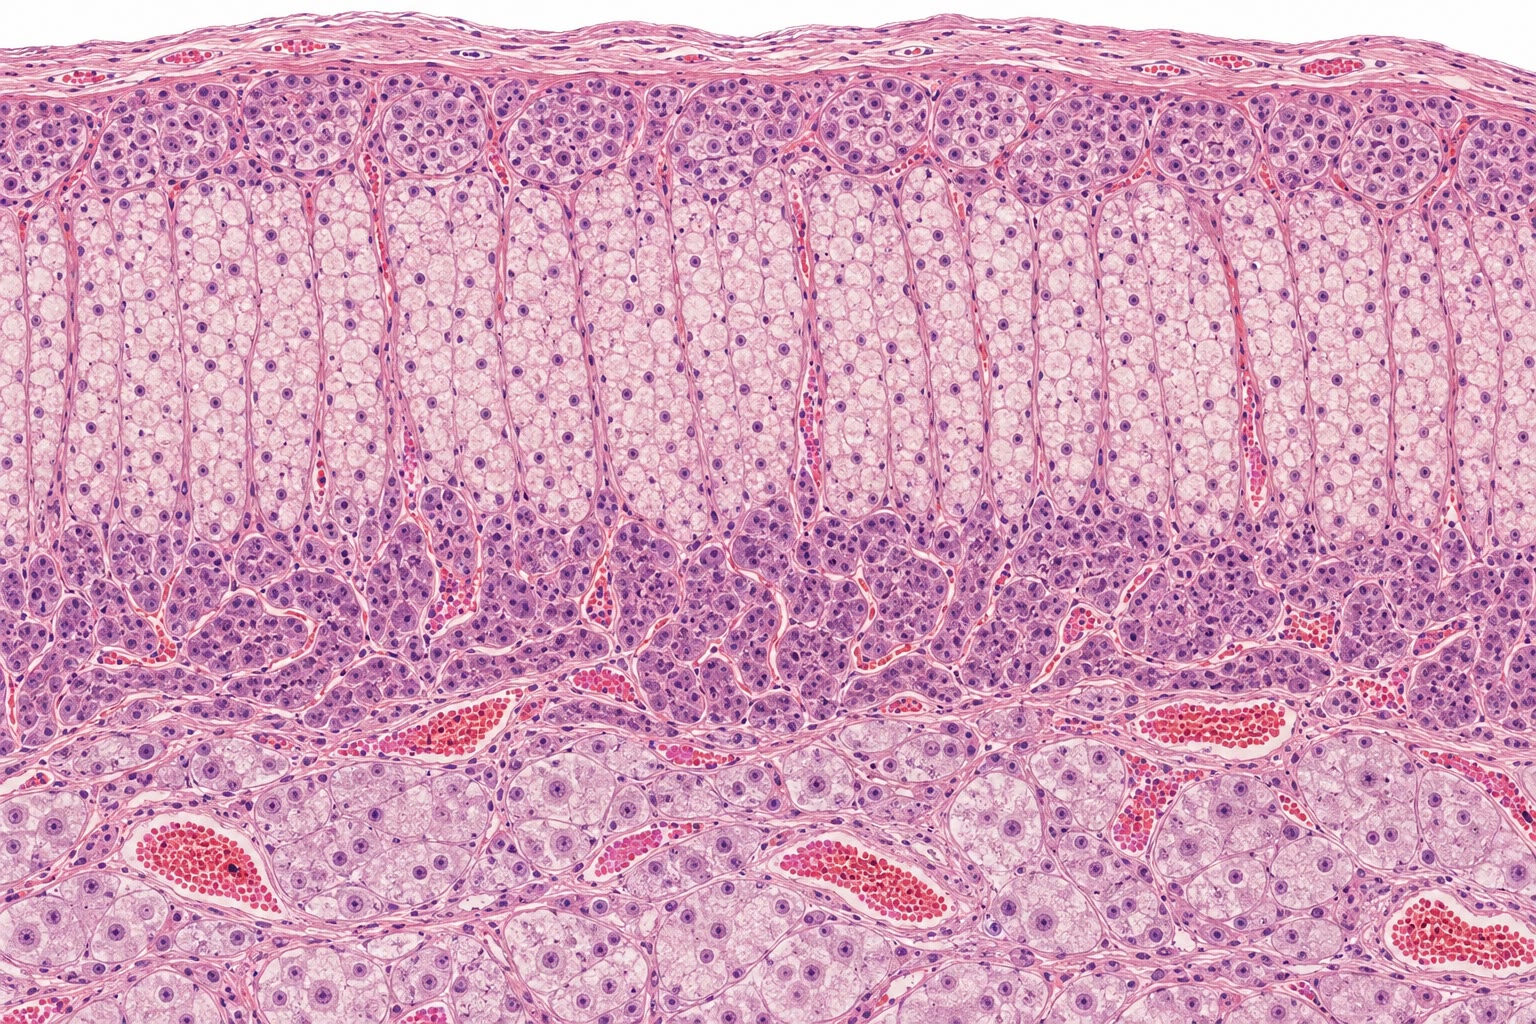
\includegraphics[width=0.5\linewidth]{images/book5/ai/b5-21-adrenal-section.jpg}\hspace{0.04\linewidth}
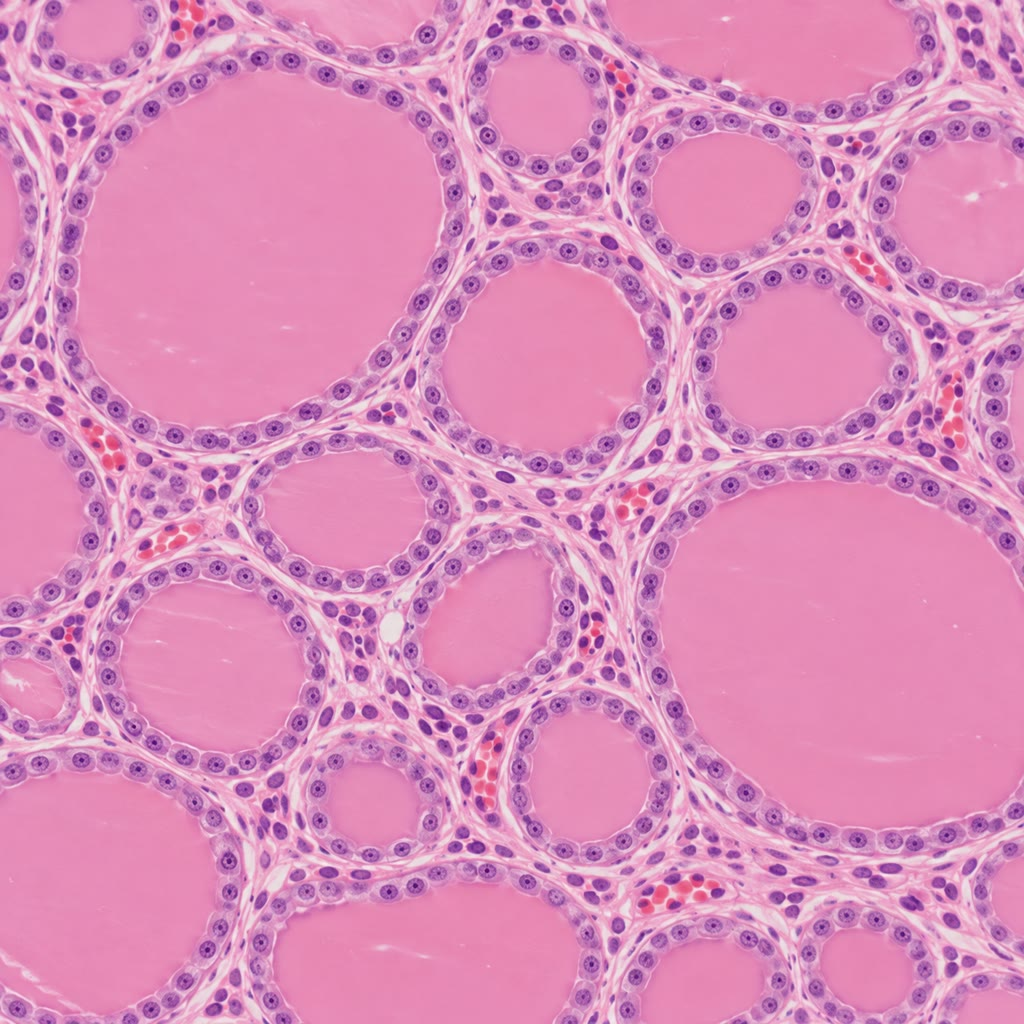
\includegraphics[width=0.36\linewidth]{images/book5/ai/b5-21-thyroid-follicles.jpg}

{\small Izquierda: la glándula suprarrenal en corte ---la corteza en
sus tres zonas (\omterm{def:b3:renal-osmoregulation:controls}{aldosterona} en la más externa, cortisol en la ancha
zona media, andrógenos en la más interna) alrededor de una médula de
células cromafines secretoras de adrenalina, que es un \omterm{def:b3:nervous-systems:comparative}{ganglio}
simpático por su origen. Derecha: folículos tiroideos, cada uno una
esfera de células en torno a un depósito de coloide que guarda \omterm{def:b3:endocrinology:hormone}{hormona}
para meses unida a la tiroglobulina.}
\end{omfigure}

\section{La glucosa: el bucle más estrecho}

\begin{definition}[Insulina y glucagón]\label{def:b3:endocrinology:glucose}
\index{insulina}\index{glucagón}\index{islote de Langerhans}\index{GLUT4}\index{diabetes mellitus}
La sangre contiene unos \qty{5}{g} de glucosa, a \qty{5}{mmol/L}
(\qty{90}{mg/dL}), y el encéfalo quema \qty{120}{g} al día y no puede
quemar otra cosa; una comida entrega \qty{75}{g} en una hora. Los
\emph{islotes de Langerhans}, un millón de grupos de unos pocos miles
de células repartidos por el páncreas, sostienen el bucle. Las células
$\beta$ detectan la glucosa metabolizándola: más glucosa, más ATP,
cierre de un canal de potasio sensible al ATP, despolarización, entrada
de calcio y exocitosis de \emph{insulina}, una \omterm{def:b3:endocrinology:hormone}{hormona peptídica}
escindida de un único precursor. La insulina dice al músculo y a la
grasa que lleven el transportador \emph{GLUT4} a su superficie y capten
glucosa, al hígado que almacene glucosa como glucógeno y deje de
fabricarla, y a la grasa que deje de liberar ácidos grasos: es la
\omterm{def:b3:endocrinology:hormone}{hormona} del estado alimentado, la única que baja la glucosa sanguínea.
Las células $\alpha$ liberan \emph{glucagón} cuando la glucosa cae: el
hígado degrada glucógeno y fabrica glucosa nueva a partir de
aminoácidos y de lactato. La adrenalina, el cortisol y la \omterm{def:b3:endocrinology:hormone}{hormona} del
crecimiento también elevan la glucosa, y la redundancia no es
simétrica: un cuerpo puede defenderse de una caída por cuatro vías y de
una subida por una sola. La \emph{diabetes mellitus} es el fallo de esa
única: la de tipo 1, la destrucción autoinmunitaria de las células
$\beta$, necesita insulina desde el primer día; la de tipo 2, nueve
casos de cada diez, empieza como resistencia de los tejidos a la
insulina, compensada durante años con más insulina, hasta que las
células $\beta$ no logran seguir el ritmo y la glucosa sube.
\end{definition}

\begin{theorem}[El bucle insulina--glucosa]\label{thm:b3:endocrinology:loop}
\index{ganancia de bucle}\index{punto de consigna}\index{oscilación amortiguada}
Escríbanse $g$ e $i$ para las desviaciones de la glucosa y de la
\omterm{def:b3:endocrinology:glucose}{insulina} plasmáticas respecto de sus valores en ayunas. La glucosa se
depura a un ritmo proporcional a su propio exceso (la eficacia de la
glucosa, $a$) y al exceso de \omterm{def:b3:endocrinology:glucose}{insulina} (la sensibilidad, $s$); la
\omterm{def:b3:endocrinology:glucose}{insulina} se segrega en proporción al exceso de glucosa ($\beta$) y se
depura a un ritmo $\gamma$; y entra una carga $u$:
\[
\dot g = -a\,g - s\,i + u, \qquad \dot i = \beta\,g - \gamma\,i .
\]
Bajo una carga constante $u$ la glucosa se asienta en
\[
g^{*} = \frac{u}{a}\cdot\frac{1}{1 + L}, \qquad L = \frac{s\beta}{a\gamma},
\]
de modo que la retroalimentación divide la perturbación que sufriría un
cuerpo sin regular entre $1 + L$, la \emph{\omterm{thm:b3:endocrinology:loop}{ganancia de bucle}} más uno.
Tras un bolo, el retorno lo gobiernan los autovalores
$\lambda = -\tfrac{a + \gamma}{2} \pm \sqrt{\tfrac{(a+\gamma)^{2}}{4} - (a\gamma + s\beta)}$:
monótono si $s\beta < (a - \gamma)^{2}/4$, y en caso contrario una
\omterm{thm:b3:endocrinology:loop}{oscilación amortiguada} de frecuencia angular $\omega = \sqrt{a\gamma + s\beta -
(a+\gamma)^{2}/4}$ que decae como $\mathrm{e}^{-(a+\gamma)t/2}$ ---la
glucosa se pasa por debajo de su valor en ayunas antes de asentarse,
que es la hipoglucemia leve de dos o tres horas después de una comida
azucarada. La resistencia a la \omterm{def:b3:endocrinology:glucose}{insulina} baja $s$: el estado
estacionario en ayunas bajo la propia producción hepática sube, y el
bucle lo compensa con un $i^{*}$ mayor, hasta que la $\beta$ de las
células $\beta$ cae también, y entonces la compensación fracasa.
\end{theorem}
\begin{proof}
Estado estacionario: $\dot i = 0$ da $i^{*} = \beta g^{*}/\gamma$; al
ponerlo en $\dot g = 0$: $a g^{*} + s\beta g^{*}/\gamma = u$, de donde $g^{*} =
u/(a + s\beta/\gamma) = (u/a)/(1 + L)$. Dinámica: la matriz del sistema
es $\begin{pmatrix} -a & -s\\ \beta & -\gamma\end{pmatrix}$, de traza
$-(a+\gamma)$ y determinante $a\gamma + s\beta$; su ecuación
característica $\lambda^{2} + (a+\gamma)\lambda + (a\gamma + s\beta) = 0$
tiene las raíces indicadas. Ambas tienen parte real negativa, de modo
que el estado de ayuno es estable; las raíces son complejas cuando el
discriminante $(a+\gamma)^{2}
- 4(a\gamma + s\beta) = (a-\gamma)^{2} - 4s\beta$ es negativo, la
condición dada, y entonces $g(t) = \mathrm{e}^{-(a+\gamma)t/2}(A\cos\omega t
+ B\sin\omega t)$, que cruza el cero. Resistencia: con $u$ igual a la
producción basal del hígado y $s$ reducida, $L$ cae y $g^{*}$ sube para
el mismo $u$; $i^{*} = \beta g^{*}/\gamma$ sube con él
(hiperinsulinemia); si $\beta$ cae después, $L$ cae más y $g^{*}$ trepa
hacia $u/a$.
\end{proof}

\begin{omfigure}
\begin{tikzpicture}
\begin{axis}[
  width=0.58\linewidth, height=5.6cm,
  axis x line=bottom, axis y line=left,
  xmin=0, xmax=180, ymin=40, ymax=200,
  xlabel={minutos tras un bolo de glucosa}, ylabel={glucosa plasmática (mg/dL)},
  xlabel style={font=\small, at={(axis description cs:0.5,-0.12)}, anchor=north}, ylabel style={font=\small},
  tick label style={font=\small}, xtick={0,30,60,90,120,150,180}, ytick={60,90,120,150,180},
  clip=false,
]
\addplot[very thick, omDef, smooth] coordinates {(0,190) (6,165) (12,131) (18,102) (24,84) (30,77) (36,78) (42,82) (48,86) (54,89) (60,91) (66,92) (72,91) (78,91) (84,90) (90,90) (96,90) (102,90) (108,90) (114,90) (120,90) (126,90) (132,90) (138,90) (144,90) (150,90) (156,90) (162,90) (168,90) (174,90) (180,90)};
\draw[dashed, gray] (axis cs:0,90) -- (axis cs:180,90);
\node[font=\scriptsize, gray, anchor=south east] at (axis cs:180,91) {nivel en ayunas};
\node[font=\scriptsize, omDef, anchor=west, align=left] at (axis cs:75,150) {modelo: $a = \qty{0.02}{min^{-1}}$, $\gamma = \qty{0.1}{min^{-1}}$,\\$s\beta = \qty{0.01}{min^{-2}}$, ganancia de bucle $L = 5$;\\mínimo por debajo a \qty{32}{min}, período \qty{68}{min}};
\node[font=\scriptsize, omThm, anchor=north] at (axis cs:24,70) {por debajo};
\end{axis}
\begin{axis}[
  at={(0.6\linewidth,0)}, anchor=south west,
  width=0.33\linewidth, height=5.6cm,
  axis x line=bottom, axis y line=left,
  xmin=0, xmax=180, ymin=0, ymax=40,
  xlabel={minutos}, ylabel={insulina (mU/L)},
  xlabel style={font=\small, at={(axis description cs:0.5,-0.12)}, anchor=north}, ylabel style={font=\small},
  tick label style={font=\small}, xtick={0,60,120,180}, ytick={0,10,20,30,40},
]
\addplot[very thick, omProp, smooth] coordinates {(0,10.0) (6,30.0) (12,33.7) (18,28.5) (24,20.4) (30,13.4) (36,8.9) (42,7.1) (48,7.1) (54,7.9) (60,9.0) (66,9.8) (72,10.2) (78,10.4) (84,10.4) (90,10.2) (96,10.1) (102,10.0) (108,10.0) (114,9.9) (120,10.0) (126,10.0) (132,10.0) (138,10.0) (144,10.0) (150,10.0) (156,10.0) (162,10.0) (168,10.0) (174,10.0) (180,10.0)};
\draw[dashed, gray] (axis cs:0,10) -- (axis cs:180,10);
\end{axis}
\end{tikzpicture}

{\small El bucle lineal tras un bolo que eleva la glucosa en
\qty{100}{mg/dL}. La \omterm{def:b3:endocrinology:glucose}{insulina} alcanza su máximo en menos de diez minutos
y la glucosa vuelve a su línea de base en veinte, y luego se pasa por
debajo; una retroalimentación fuerte que actúa mediante una \omterm{def:b3:endocrinology:hormone}{hormona} con
su propio tiempo de depuración regresa como una \omterm{thm:b3:endocrinology:loop}{oscilación amortiguada}
y no como una simple caída.}
\end{omfigure}

\begin{proof}[Evidencia]
Von Mering y Minkowski (1889) extirparon el páncreas a un perro y
produjeron diabetes ---las moscas que se juntaban sobre su orina
delataron el azúcar; ligar los conductos, que destruía el tejido
digestivo pero respetaba los islotes, no la producía. Banting y Best
(1921), con la purificación de Collip, extrajeron el principio de los
islotes y bajaron el azúcar de un perro diabético, y después el de
Leonard Thompson (enero de 1922). Sanger secuenció la \omterm{def:b3:endocrinology:glucose}{insulina} (1955),
la primera secuencia de una proteína; Yalow y Berson la midieron en
sangre (1959) y hallaron que los diabéticos de comienzo adulto tenían,
al principio, más que los sanos ---resistencia, no carencia. Las
bacterias de Genentech fabricaron \omterm{def:b3:endocrinology:glucose}{insulina} humana en 1978, el primer
fármaco recombinante.
\end{proof}

\begin{omfigure}
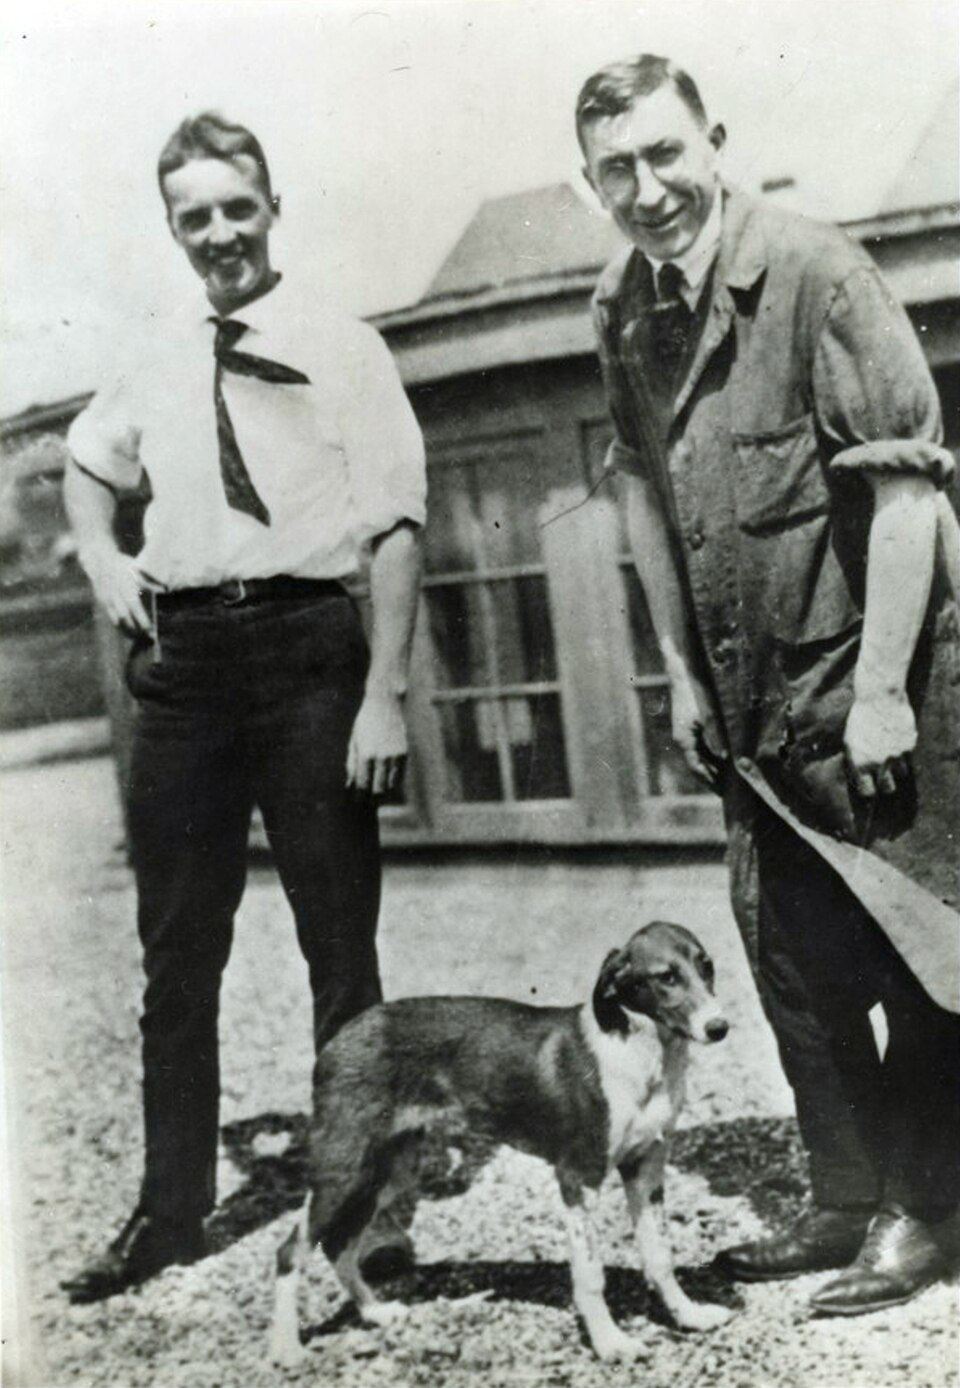
\includegraphics[width=0.42\linewidth]{images/book5/banting-best.jpg}\hspace{0.04\linewidth}
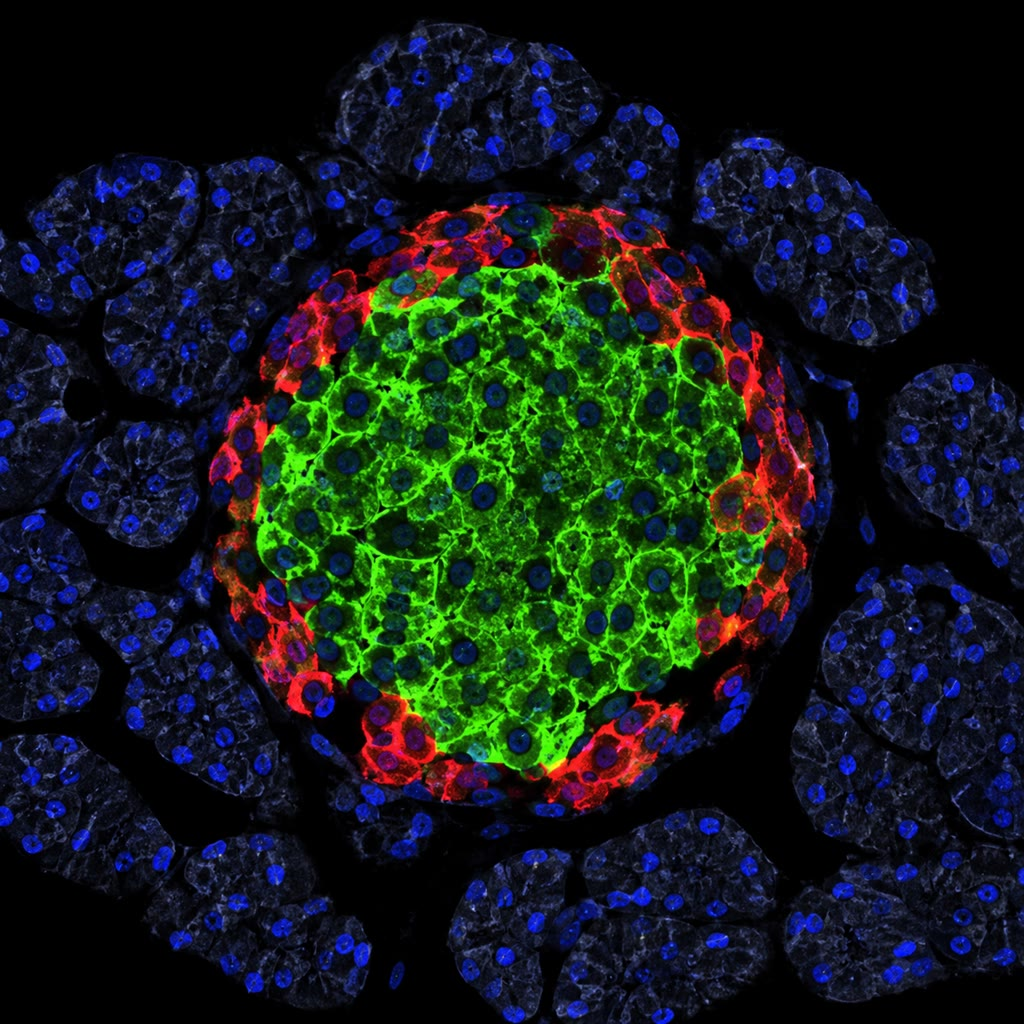
\includegraphics[width=0.42\linewidth]{images/book5/ai/b5-21-pancreatic-islet.jpg}

{\small Izquierda: Frederick Banting y Charles Best en el tejado del
edificio de medicina de Toronto, hacia 1924, con uno de los perros de
los experimentos de la \omterm{def:b3:endocrinology:glucose}{insulina} (fotografía de dominio público).
Derecha: un \omterm{def:b3:endocrinology:glucose}{islote de Langerhans}, con las células $\beta$ productoras
de \omterm{def:b3:endocrinology:glucose}{insulina} en el núcleo y las células $\alpha$ del \omterm{def:b3:endocrinology:glucose}{glucagón} en el
borde, en un mar de acinos exocrinos.}
\end{omfigure}

\begin{method}[Leer el bucle de la glucosa en un paciente]\label{met:b3:endocrinology:ogtt}
\index{prueba de tolerancia a la glucosa}\index{HbA1c}
(1) Glucosa plasmática en ayunas: normal por debajo de
\qty{5.6}{mmol/L}, diabetes en \qty{7.0}{mmol/L} o por encima en dos
ocasiones. (2) Prueba de tolerancia oral a la glucosa: se beben
\qty{75}{g} de glucosa; la glucosa plasmática a las dos horas es normal
por debajo de \qty{7.8}{mmol/L} y diabética en \qty{11.1}{mmol/L} o por
encima ---el valor de las dos horas lee la ganancia del bucle; el de
ayunas, su \omterm{thm:b3:endocrinology:loop}{punto de consigna}. (3) Hemoglobina glucosilada,
\emph{HbA1c}: la glucosa se fija de forma irreversible a la hemoglobina
a un ritmo proporcional a su concentración, y los glóbulos rojos viven
120 días, de modo que la fracción glucosilada integra la glucosa media
de los tres meses anteriores sin necesidad de ayuno ---normal por
debajo del \qty{5.7}{\%}, diabética desde el \qty{6.5}{\%}. (4) Para
separar la resistencia de la carencia, mídase la \omterm{def:b3:endocrinology:glucose}{insulina} (o su
subproducto, el péptido~C) al lado: \omterm{def:b3:endocrinology:glucose}{insulina} alta con glucosa alta es
resistencia; péptido~C ausente es tipo~1.
\end{method}

\section{El calcio, y el reloj}

\begin{definition}[La homeostasis del calcio]\label{def:b3:endocrinology:calcium}
\index{hormona paratiroidea}\index{calcitriol}\index{vitamina D}\index{osteoporosis}
El calcio ionizado del plasma se mantiene en \qty{1.2}{mmol/L} con un
margen de un pequeño porcentaje, porque fija la excitabilidad de todo
nervio y todo músculo: si es demasiado bajo descargan espontáneamente
(tetania), y si es demasiado alto se vuelven perezosos. Las cuatro
glándulas paratiroides lo detectan con un receptor de superficie y
segregan \emph{\omterm{def:b3:endocrinology:hormone}{hormona} paratiroidea} (PTH) a lo largo de una sigmoide
inversa muy inclinada: la PTH moviliza calcio del hueso, hace que el
riñón lo reabsorba y excrete fosfato, y activa la \emph{vitamina D}
---fabricada en la piel por la luz ultravioleta o comida, hidroxilada
en el hígado y luego en el riñón hasta \emph{calcitriol}---, que hace
que el intestino absorba calcio. El hueso es el depósito, un kilogramo
de calcio, remodelado sin cesar por osteoclastos y osteoblastos bajo la
PTH, el calcitriol, los estrógenos y la carga. La carencia de vitamina
D da raquitismo en los niños y huesos blandos en los adultos; la caída
de los estrógenos en la menopausia inclina la remodelación hacia la
resorción y da \emph{osteoporosis}; un adenoma paratiroideo eleva el
calcio, disuelve el hueso y forma cálculos renales ---``huesos, piedras
y quejidos''.
\end{definition}

\begin{definition}[El reloj circadiano]\label{def:b3:endocrinology:clock}
\index{reloj circadiano}\index{núcleo supraquiasmático}\index{genes reloj}\index{melatonina}\index{zeitgeber}
Casi toda célula lleva un \emph{reloj circadiano}: un bucle de
transcripción y traducción en el que las proteínas CLOCK y BMAL1
encienden los genes \emph{Per} y \emph{Cry}, cuyas proteínas se
acumulan, entran en el núcleo tras un retraso de horas y reprimen su
propia transcripción, y luego se degradan y levantan la represión ---un
ciclo en unas veinticuatro horas, fijado por las velocidades del
retraso y de la degradación. Los relojes del cuerpo los sincroniza un
reloj maestro de veinte mil neuronas del \emph{núcleo supraquiasmático}
del \omterm{def:b3:endocrinology:axes}{hipotálamo}, que la luz pone en hora a través de una clase
específica de \omterm{def:b3:sensory-systems:retina}{células ganglionares} de la \omterm{def:b3:sensory-systems:retina}{retina} (que contienen
melanopsina y no los pigmentos de los bastones ni de los \omterm{def:b3:sensory-systems:retina}{conos}), y que
anuncia la noche al cuerpo mediante la \emph{melatonina} de la pineal,
segregada solo en la oscuridad. El reloj programa el cortisol antes de
despertar, la temperatura corporal más baja a las cuatro de la
madrugada, la \omterm{def:b3:endocrinology:hormone}{hormona} del crecimiento en el primer sueño, la
sensibilidad a la \omterm{def:b3:endocrinology:glucose}{insulina} más alta por la mañana; la comida, el
ejercicio y la temperatura son \emph{zeitgebers} secundarios que pueden
apartar los relojes periféricos del central, que es el malestar del
trabajador por turnos y del desfase horario ---un reloj hepático en una
hora y un encéfalo en otra.
\end{definition}

\begin{proof}[Evidencia]
Konopka y Benzer (1971) cribaron moscas mutantes en busca de ritmos de
emergencia alterados y hallaron tres alelos de un solo gen,
\emph{period}: un día corto (19 h), un día largo (29 h) y ausencia
total de ritmo ---un reloj con un período genético. Hardin, Hall y
Rosbash (1990) hallaron que el ARNm y la proteína de \emph{period}
oscilan con un desfase entre ambos, y que la proteína reprime su propio
gen: el bucle. Ralph y Menaker (1990) trasplantaron el \omterm{def:b3:endocrinology:clock}{núcleo
supraquiasmático} de un hámster mutante de ritmo de 20 horas a un
hámster normal cuyo propio núcleo había sido destruido: el receptor
pasó a funcionar con 20 horas ---el período pertenecía al tejido
trasplantado. En personas mantenidas en un búnker sin señales horarias
el ritmo corría libre en algo más de 24 horas; una luz intensa por la
tarde lo retrasaba, y por la mañana lo adelantaba.
\end{proof}

\begin{omfigure}
\begin{tikzpicture}[every node/.style={font=\scriptsize}, >=stealth]
  \node[draw, thick, rounded corners, fill=omDef!20, align=center] (cb) at (0,1.6) {activadores\\CLOCK--BMAL1};
  \node[draw, thick, rounded corners, fill=omProp!25, align=center] (pc) at (3.6,1.6) {\emph{Per}, \emph{Cry}\\transcritos};
  \node[draw, thick, rounded corners, fill=omThm!20, align=center] (pr) at (3.6,-0.4) {las proteínas PER y CRY\\se acumulan y dimerizan};
  \node[draw, thick, rounded corners, fill=omMeth!25, align=center] (nu) at (0,-0.4) {entran en el núcleo\\tras unas horas};
  \draw[->, thick] (cb) -- (pc) node[midway, above, font=\tiny] {activan};
  \draw[->, thick] (pc) -- (pr) node[midway, right, font=\tiny] {traducción, retraso};
  \draw[->, thick] (pr) -- (nu);
  \draw[-|, thick, omThm] (nu) -- (cb) node[midway, left, font=\tiny, omThm, align=right] {reprimen\\a sus propios\\activadores};
  \draw[->, thick, gray] (nu.south) -- ++(0,-0.5) node[below, font=\tiny, gray, align=center] {degradadas: se levanta la represión;\\el ciclo recomienza, $\approx$ \qty{24}{h}};
  % right: daily profile
  \begin{scope}[shift={(7.2,-1.6)}]
    \draw[->] (0,0) -- (5.6,0) node[right, font=\tiny] {hora};
    \draw[->] (0,0) -- (0,3.4);
    \foreach \x/\l in {0/0, 1.4/6, 2.8/12, 4.2/18, 5.6/24} { \draw (\x,0) -- (\x,-0.08) node[below, font=\tiny] {\l}; }
    \fill[gray!25] (0,0) rectangle (1.4,3.4); \fill[gray!25] (5.1,0) rectangle (5.6,3.4);
    \node[font=\tiny, gray!60!black] at (0.7,3.2) {noche};
    \draw[very thick, omMeth!70!black, domain=0:5.6, samples=60, smooth, variable=\x] plot (\x, {1.6 + 1.2*cos(deg(2*3.1416*(\x-1.9)/5.6))});
    \node[font=\tiny, omMeth!70!black] at (3.1,3.1) {cortisol: máximo a las 8};
    \draw[very thick, omDef, domain=0:5.6, samples=60, smooth, variable=\x] plot (\x, {0.9 + 0.7*cos(deg(2*3.1416*(\x-0.7)/5.6))});
    \node[font=\tiny, omDef] at (2.7,0.18) {melatonina: solo de noche};
  \end{scope}
\end{tikzpicture}

{\small Izquierda: el núcleo del reloj molecular, un bucle de
\omterm{def:b3:endocrinology:axes}{retroalimentación negativa} con un retraso de horas, que es lo que un
bucle necesita para oscilar en lugar de asentarse. Derecha: dos
\omterm{def:b3:endocrinology:hormone}{hormonas} que programa ---el cortisol, que sube antes del amanecer para
preparar el día, y la \omterm{def:b3:endocrinology:clock}{melatonina}, que marca la noche.}
\end{omfigure}

\begin{remark}[La homeostasis como control]\label{rem:b3:endocrinology:control}
Todos los bucles de este capítulo tienen las mismas piezas: un sensor
(el metabolismo de la célula $\beta$, el receptor de calcio de la
paratiroides, el receptor de \omterm{prop:b3:endocrinology:thyroid}{hormona tiroidea} de la \omterm{def:b3:endocrinology:axes}{hipófisis}), un
controlador que compara con un \omterm{thm:b3:endocrinology:loop}{punto de consigna}, una \omterm{def:b3:endocrinology:hormone}{hormona} efectora
con su propia semivida, y una retroalimentación que reduce el error en
un factor $1 + L$ pero nunca hasta cero. Lo que cambia es el tiempo
---segundos para la adrenalina, una hora para la \omterm{def:b3:endocrinology:glucose}{insulina}, días para la
tiroxina, toda una vida para el hueso--- y el precio del compromiso: un
bucle rápido con un efector retrasado oscila, y un bucle lento deja que
una perturbación persista. La clínica ve los bucles desde fuera, a
través de los pares que la retroalimentación acopla: una TSH alta con
una T$_{4}$ baja es una glándula que ha fallado, y una TSH alta con una
T$_{4}$ alta, una \omterm{def:b3:endocrinology:axes}{hipófisis} que ha fallado; una \omterm{def:b3:endocrinology:glucose}{insulina} alta con una
glucosa alta es resistencia, y una \omterm{def:b3:endocrinology:glucose}{insulina} baja con una glucosa alta,
destrucción. Para leer el nivel de una \omterm{def:b3:endocrinology:hormone}{hormona} siempre hay que
preguntar qué estaba haciendo su superior.
\end{remark}

\section{Ejercicios}

\begin{exercise}[$\star$]\label{exo:b3:endocrinology:1}
Clasifíquense la \omterm{def:b3:endocrinology:glucose}{insulina}, el cortisol, la adrenalina, la tiroxina y la
vasopresina por su química, la localización del receptor, la rapidez de
acción y la semivida.
\end{exercise}

\begin{exercise}[$\star$]\label{exo:b3:endocrinology:2}
Dibújese el eje tiroideo con su retroalimentación y predíganse la TSH y
la T$_{4}$ en: una tiroides destruida; un \omterm{def:b3:cancer-biology:hallmarks}{tumor} hipofisario secretor de
TSH; un paciente que toma demasiada tiroxina; una carencia de yodo.
\end{exercise}

\begin{exercise}[$\star$]\label{exo:b3:endocrinology:3}
¿Por qué tiene un cuerpo cuatro \omterm{def:b3:endocrinology:hormone}{hormonas} que elevan la glucosa
sanguínea y solo una que la baja? ¿Qué predice esto sobre los peligros
relativos de un exceso y de un defecto de \omterm{def:b3:endocrinology:glucose}{insulina}?
\end{exercise}

\begin{exercise}[$\star$]\label{exo:b3:endocrinology:4}
¿Qué es un \omterm{def:b3:endocrinology:clock}{zeitgeber}? Dense tres, dígase cuál emplea el reloj maestro y
explíquese qué le ocurre a un viajero que cruza ocho husos horarios.
\end{exercise}

\begin{exercise}[$\star\star$]\label{exo:b3:endocrinology:5}
Una célula tiene \num{20000} receptores con $K_{d} = \qty{1}{nM}$ y
responde al máximo cuando hay \num{500} ocupados. Hállese la
EC$_{50}$. Tras una semana de \omterm{def:b3:endocrinology:hormone}{hormona} alta la célula tiene \num{2000}
receptores: ¿nueva EC$_{50}$? Interprétese para la resistencia a la
\omterm{def:b3:endocrinology:glucose}{insulina}.
\end{exercise}

\begin{exercise}[$\star\star$]\label{exo:b3:endocrinology:6}
Con $\kappa = \qty{0.46}{L/pmol}$ y una TSH normal de \qty{1.5}{mU/L}
para una T$_{4}$ libre de \qty{15}{pmol/L}, calcúlese la TSH cuando la
T$_{4}$ vale $13$, $11$, $9$ y \qty{25}{pmol/L}. ¿En cuáles de estos
casos seguiría la T$_{4}$ dentro de un intervalo de referencia de
\qtyrange{10}{20}{pmol/L} mientras la TSH queda fuera de
\qtyrange{0.4}{4}{mU/L}?
\end{exercise}

\begin{exercise}[$\star\star$]\label{exo:b3:endocrinology:7}
En el bucle de \cref{thm:b3:endocrinology:loop} con $a = \qty{0.02}{min^{-1}}$,
$\gamma = \qty{0.1}{min^{-1}}$, $\beta = \qty{0.05}{mU\,L^{-1}\,min^{-1}}$
por mg/dL y $s = \qty{0.2}{mg\,dL^{-1}\,min^{-1}}$ por mU/L, calcúlense
la \omterm{thm:b3:endocrinology:loop}{ganancia de bucle}, el exceso estacionario de glucosa bajo una carga
constante de \qty{2}{mg/dL/min}, el mismo sin retroalimentación y el
exceso estacionario de \omterm{def:b3:endocrinology:glucose}{insulina}.
\end{exercise}

\begin{exercise}[$\star\star$]\label{exo:b3:endocrinology:8}
Con los mismos parámetros: ¿es oscilatorio el retorno tras un bolo?
Calcúlense el período y el tiempo que tarda la amplitud en caer en un
factor $\mathrm{e}$. Redúzcase ahora $s$ a la mitad (resistencia a la
\omterm{def:b3:endocrinology:glucose}{insulina}): recalcúlense ambos y la nueva \omterm{thm:b3:endocrinology:loop}{ganancia de bucle}.
\end{exercise}

\begin{exercise}[$\star\star$]\label{exo:b3:endocrinology:9}
La semivida del cortisol es de \qty{80}{min}. Un paciente que toma
\qty{40}{mg} de prednisolona al día durante un año lo interrumpe de
golpe. Explíquese, piso por piso, por qué puede colapsarse ante una
infección menor tres días después, y qué mostraría el eje si se midiera
(ACTH, cortisol, respuesta a la ACTH inyectada).
\end{exercise}

\begin{exercise}[$\star\star\star$]\label{exo:b3:endocrinology:10}
Muéstrese que una \omterm{def:b3:endocrinology:axes}{retroalimentación negativa} de una sola variable
$\dot x = f(x)$ con $f' < 0$ no puede oscilar, mientras que el bucle de
dos variables del teorema sí, y explíquese con palabras por qué el
reloj necesita un retraso de horas entre la transcripción y la
represión para dar un período de 24 horas. ¿Qué le ocurriría al período
si PER se degradara al doble de velocidad?
\end{exercise}

\begin{exercise}[$\star\star\star$]\label{exo:b3:endocrinology:11}
La \omterm{def:b3:endocrinology:calcium}{hormona paratiroidea} sigue $\text{PTH} = P_{\max}/(1 +
\mathrm{e}^{k(\text{Ca} - \text{Ca}_{0})})$ con $\text{Ca}_{0} =
\qty{1.2}{mmol/L}$ y $k = \qty{20}{L/mmol}$. Calcúlese la PTH como
fracción del máximo para Ca $= 1.10$, $1.15$, $1.20$, $1.25$ y
\qty{1.30}{mmol/L}, y la pendiente en el \omterm{thm:b3:endocrinology:loop}{punto de consigna}, y
explíquese por qué una inclinación así conviene para el calcio pero
sería peligrosa para la glucosa.
\end{exercise}

\begin{exercise}[$\star\star\star$]\label{exo:b3:endocrinology:12}
La glucosa se fija a la hemoglobina a un ritmo $k\,G$ por unidad de
tiempo, con una $k$ tal que una glucosa media de \qty{5.5}{mmol/L} da
un \qty{5}{\%} de glucosilación a lo largo de los 120 días de vida de
un glóbulo rojo. Dedúzcase la HbA1c en función de la glucosa media y su
valor a \qty{10}{mmol/L}, y explíquese por qué un paciente con una
anemia hemolítica (glóbulos rojos que viven 60 días) tiene una HbA1c
engañosamente baja.
\end{exercise}

\section{Problema: el azúcar de la sangre}

\begin{problem}[{Problema de fin de semana --- una \omterm{met:b3:endocrinology:ogtt}{prueba de tolerancia
a la glucosa} leída a través del bucle lineal insulina--glucosa: la
distribución de una dosis de \qty{75}{g}, la \omterm{thm:b3:endocrinology:loop}{ganancia de bucle} y el
retorno amortiguado, lo que la resistencia y el fallo de las células
$\beta$ hacen al \omterm{thm:b3:endocrinology:loop}{punto de consigna} en ayunas, un diagnóstico a partir
de los números y el eje tiroideo al lado, para terminar en la \omterm{thm:b3:endocrinology:loop}{ganancia
de bucle}, el tiempo de retorno y la glucosa en ayunas del bucle que
falla}]
\label{pb:b3:endocrinology:1}
Datos: un adulto sano, volumen de distribución de la glucosa
\qty{15}{L}, glucosa en ayunas \qty{90}{mg/dL} (\qty{5}{mmol/L}),
\omterm{def:b3:endocrinology:glucose}{insulina} en ayunas \qty{10}{mU/L}. Parámetros del bucle:
$a = \qty{0.02}{min^{-1}}$, $\gamma =
\qty{0.1}{min^{-1}}$, $\beta = 0.05$ (mU/L por min y por mg/dL),
$s = 0.2$ (mg/dL por min y por mU/L). Producción hepática basal de
glucosa $u_{0} =
\qty{2}{mg/dL/min}$ (ya equilibrada en el estado de ayuno por la
eliminación en ayunas). Una dosis oral de \qty{75}{g} se absorbe a lo
largo de una hora. Tiroides:
$\text{TSH} = 1.5\,\mathrm{e}^{-0.46(T_{4} - 15)}$ mU/L. Masa molar de
la glucosa, \qty{180}{g/mol}.

\medskip
\noindent\textbf{Parte I --- La dosis.}
\begin{enumerate}
  \item Exprésese la glucosa en ayunas en mmol/L y compruébese la
        conversión desde mg/dL. ¿Cuántos gramos de glucosa hay en el
        volumen de distribución en ayunas?
  \item Si los \qty{75}{g} enteros apareciesen de golpe en \qty{15}{L},
        ¿cuánto subiría la glucosa (en mg/dL y en mmol/L)? ¿Por qué el
        máximo real, de unos \qty{60}{mg/dL} por encima del ayuno, se
        queda tan corto?
  \item Absorbida a lo largo de \qty{60}{min}, ¿a qué ritmo entra la
        dosis, en mg/dL por minuto? Compárese con $u_{0}$.
  \item Sin respuesta alguna de \omterm{def:b3:endocrinology:glucose}{insulina} ($s = 0$), la glucosa
        obedecería $\dot
        g = -a g + u$. Exceso estacionario bajo el ritmo de absorción y
        constante de tiempo de la aproximación. ¿Dónde estaría la
        glucosa al cabo de una hora?
  \item Con el bucle, calcúlense $L$ y el exceso estacionario bajo el
        mismo ritmo. Compárese con la pregunta~4.
  \item Explíquese por qué el encéfalo está protegido por ambos lados:
        qué necesita, y qué hace a los tejidos, a lo largo de los años,
        un exceso de glucosa.
\end{enumerate}

\medskip
\noindent\textbf{Parte II --- El retorno.}
\begin{enumerate}[resume]
  \item Escríbase la ecuación característica del bucle y calcúlense la
        traza, el determinante y el discriminante.
  \item Calcúlense $\omega$ y el período de la \omterm{thm:b3:endocrinology:loop}{oscilación amortiguada},
        y el tiempo de decaimiento $2/(a + \gamma)$.
  \item Partiendo de un exceso de \qty{100}{mg/dL} con la \omterm{def:b3:endocrinology:glucose}{insulina} en su
        valor de ayunas, la solución es $g(t) = 100\,\mathrm{e}^{-0.06t}
        (\cos\omega t + c\sin\omega t)$. Hállese $c$ a partir de $\dot g(0) = -a\cdot
        100$.
  \item ¿Cuándo vuelve la glucosa por primera vez al valor de ayunas
        (primer cero de $g$)? Estímese cuánto baja por debajo en el
        primer mínimo.
  \item \omterm{def:b3:endocrinology:glucose}{Insulina}: $i(t)$ tiene la misma exponencial y la misma
        frecuencia. Arguméntese a partir de $\dot i = \beta g - \gamma i$
        que su máximo llega después de que la glucosa haya empezado a
        caer y antes de que la glucosa alcance el valor de ayunas.
  \item ¿Por qué una prueba de tolerancia real, con una absorción de una
        hora y no un bolo, muestra un máximo a los 30--60 minutos y un
        retorno a las dos horas, y solo un leve descenso a las tres?
\end{enumerate}

\medskip
\noindent\textbf{Parte III --- Cuando el bucle falla.}
\begin{enumerate}[resume]
  \item La resistencia a la \omterm{def:b3:endocrinology:glucose}{insulina} reduce $s$ a la mitad. ¿Nueva $L$?
        La $u_{0}$ del hígado la atiende ahora un nuevo estado
        estacionario de ayuno: empleando $g^{*} = (u_{0}/a)/(1
        + L)$ como el exceso sobre una línea de base idealizada sin
        regular, hállese cuánto sube la glucosa en ayunas respecto del
        estado sano (calcúlense ambos valores de $g^{*}$ y réstense).
  \item \omterm{def:b3:endocrinology:glucose}{Insulina} en ayunas en el estado resistente: calcúlese $i^{*} = \beta
        g^{*}/\gamma$ para ambos estados y la razón entre ellos. ¿Cómo
        llama la clínica a esto?
  \item Ahora fallan las células $\beta$: $\beta$ cae también a la
        quinta parte. Nueva $L$, nuevo exceso en ayunas. Conviértase a
        mmol/L y compárese con el umbral diabético de \qty{7}{mmol/L}.
  \item ¿Sigue siendo oscilatorio el retorno en el estado de la
        pregunta~15? Calcúlense el discriminante y la constante de
        tiempo del modo más lento.
  \item Un paciente tiene una glucosa en ayunas de \qty{8}{mmol/L}, una
        \omterm{def:b3:endocrinology:glucose}{insulina} en ayunas de \qty{30}{mU/L} y un valor a las dos horas
        de \qty{13}{mmol/L}. Diagnostíquense el tipo y el mecanismo a
        partir de los pares.
  \item Otro tiene una glucosa en ayunas de \qty{15}{mmol/L}, un
        péptido~C indetectable y ha perdido \qty{8}{kg} en dos meses.
        Diagnostíquese, y explíquese la pérdida de peso en términos de
        lo que hacen los tejidos sin \omterm{def:b3:endocrinology:glucose}{insulina}.
  \item HbA1c: si la glucosa media del primer paciente es de
        \qty{9}{mmol/L}, y \qty{5.5}{mmol/L} da un \qty{5}{\%}, estímese
        su HbA1c suponiendo proporcionalidad.
\end{enumerate}

\medskip
\noindent\textbf{Parte IV --- La glándula de al lado.}
\begin{enumerate}[resume]
  \item La T$_{4}$ libre es de \qty{12}{pmol/L}. Calcúlese la TSH. ¿Está
        la T$_{4}$ en el intervalo \qtyrange{10}{20}{pmol/L}? ¿Está la
        TSH en \qtyrange{0.4}{4}{mU/L}? ¿Cómo se llama ese estado?
  \item La T$_{4}$ vale \qty{7}{pmol/L}: ¿TSH? Un paciente con esta
        T$_{4}$ pero una TSH de \qty{0.3}{mU/L}: ¿dónde está la lesión?
  \item La semivida de la tiroxina es de \qty{7}{d}. Un paciente en
        tratamiento sustitutivo olvida las pastillas de una semana. ¿A
        qué fracción cae el nivel, y por qué es la semana olvidada menos
        peligrosa que un día olvidado de reposición de cortisol?
  \item Enfermedad de Graves: un \omterm{def:b3:adaptive-immunity:antibody}{anticuerpo} ocupa el receptor de TSH.
        Predíganse la T$_{4}$, la TSH y el efecto de la relación
        log-lineal sobre la TSH medida.
  \item Explíquese en un párrafo por qué el nivel de una \omterm{def:b3:endocrinology:hormone}{hormona} carece
        de sentido sin el nivel de quien la manda, empleando los cuatro
        pares de la última observación del capítulo.
  \item Resúmase: la \omterm{thm:b3:endocrinology:loop}{ganancia de bucle} sana (pregunta~5), el período y
        el tiempo de decaimiento del retorno (pregunta~8) y la glucosa
        en ayunas del bucle que falla (pregunta~15).
\end{enumerate}
\end{problem}
